\documentclass[11pt]{article}
\usepackage[a4paper,left=2.3cm,right=2.3cm,top=2.2cm,bottom=2.4cm]{geometry}
\usepackage{amsmath}
\usepackage{fontspec}
\usepackage{unicode-math}
\setmainfont{texgyrepagella}[Extension=.otf,UprightFont=*-regular,BoldFont=*-bold,ItalicFont=*-italic,BoldItalicFont=*-bolditalic]
\setsansfont{texgyreheros}[Extension=.otf,UprightFont=*-regular,BoldFont=*-bold,ItalicFont=*-italic,BoldItalicFont=*-bolditalic]
\setmathfont{texgyrepagella-math.otf}
\usepackage{xcolor}
\usepackage{tikz}
\usetikzlibrary{arrows.meta,positioning,patterns,calc,shapes.geometric,decorations.pathreplacing}
\usepackage[most]{tcolorbox}
\usepackage{booktabs,array,tabularx,enumitem}
\usepackage{titlesec}
\usepackage[hidelinks]{hyperref}
\usepackage{fancyhdr}

\definecolor{ana}{HTML}{0F5257}
\definecolor{kum}{HTML}{F4EFE6}
\definecolor{tur}{HTML}{E3F1EF}
\definecolor{uyari}{HTML}{FBEDE3}
\definecolor{turuncu}{HTML}{D9822B}
\definecolor{gri}{HTML}{5F6B6D}

\titleformat{\section}{\sffamily\Large\bfseries\color{ana}}{\thesection}{0.6em}{}
\titlespacing*{\section}{0pt}{16pt}{6pt}
\titleformat{\subsection}{\sffamily\large\bfseries\color{ana}}{}{0em}{}
\titlespacing*{\subsection}{0pt}{10pt}{4pt}

\newtcolorbox{ozet}{enhanced,colback=kum,colframe=kum,arc=3pt,left=12pt,right=12pt,top=10pt,bottom=10pt}
\newtcolorbox{sonuc}{enhanced,colback=tur,colframe=ana,boxrule=0.8pt,arc=3pt,left=12pt,right=12pt,top=9pt,bottom=9pt}
\newtcolorbox{sezgi}[1][]{colback=tur,colframe=ana,boxrule=0pt,leftrule=3pt,arc=0pt,
  fonttitle=\sffamily\bfseries\small,coltitle=ana,title={#1},attach title to upper={\ \ },left=9pt,right=9pt,top=6pt,bottom=6pt}
\newtcolorbox{dikkat}[1][]{colback=uyari,colframe=turuncu,boxrule=0pt,leftrule=3pt,arc=0pt,
  fonttitle=\sffamily\bfseries\small,coltitle=turuncu!70!black,title={#1},attach title to upper={\ \ },left=9pt,right=9pt,top=6pt,bottom=6pt}

\setlength{\emergencystretch}{3em}
\setlength{\parskip}{5pt}
\setlength{\parindent}{0pt}
\setlist{itemsep=2pt,topsep=3pt}
\renewcommand{\figurename}{Şekil}

\pagestyle{fancy}
\fancyhf{}
\renewcommand{\headrulewidth}{0pt}
\fancyfoot[L]{\sffamily\footnotesize\color{gri}Qplex'ler ne kadar ileri gidebilir? \,·\, Herkes için özet}
\fancyfoot[R]{\sffamily\footnotesize\color{gri}\thepage}

\hypersetup{pdftitle={Qplex'ler ne kadar ileri gidebilir? Herkes için özet},pdfauthor={Yusuf Kaan Öğüt}}

\begin{document}
\thispagestyle{fancy}

\begin{tcolorbox}[enhanced,colback=ana,colframe=ana,arc=4pt,left=16pt,right=16pt,top=14pt,bottom=14pt]
\color{white}
{\sffamily\small HERKES İÇİN ÖZET}\\[6pt]
{\sffamily\bfseries\huge Qplex'ler ne kadar ileri gidebilir?}\\[6pt]
{\large Kuantum fiziğinin temellerindeki açık bir sorunun cevabı}\\[10pt]
{\sffamily\bfseries Yusuf Kaan Öğüt}{\sffamily\small \;·\; 25 Kasım 2026}\\[2pt]
{\sffamily\small Yapay zekâ katkısı: Claude Opus 5.5 (Anthropic) ve OpenAI Codex (GPT-6.2 Astra)}
\end{tcolorbox}

\vspace{4pt}
\begin{ozet}
{\sffamily\bfseries\color{ana} Kısaca.}
Fizikçiler Sachin Gupta ve Jacques Pienaar 2026'da şunu gösterdi: Kuantum mekaniğini olasılıkların
geometrisinden yeniden kurmaya çalışan \emph{qplex} modelleri, CGLMP adlı bir Bell testinde kuantum
mekaniğinin izin verdiğinden daha yüksek bir puana, yaklaşık 3,155'e ulaşabiliyor. Bundan da yükseğe
çıkılıp çıkılamayacağını ise bilmiyorlardı. Makalelerinde bunu açık bir soru olarak bıraktılar ve
çıkılamayacağını tahmin ettiler. Bu çalışma o tahmini kanıtlıyor: qplex modelleri bu testte
$2+2/\sqrt3\approx3{,}1547$'yi \textbf{hiçbir koşulda} geçemez. Kanıtın bir kısmı kâğıt kalemle yapıldı. En
zor kısmı ise herkesin yaklaşık 35 saniyede yeniden çalıştırabileceği, yuvarlama hatası içermeyen bir
bilgisayar kontrolüne dayanıyor.
\end{ozet}

%==========================================================
\section{Bir oyunla başlayalım: Bell testleri}

Alice ile Bob'u ayrı odalara koyduğumuzu düşünelim. Her turda ikisine de iki sorudan biri soruluyor
(“0” ya da “1”) ve her biri üç cevaptan birini veriyor (“0”, “1” ya da “2”). Oyun sırasında
haberleşemiyorlar, ama oyundan önce istedikleri stratejiyi kararlaştırabiliyorlar. Bir hakem, soruların
hangi çifte denk geldiğine göre cevaplarının \emph{farkına} bakıp puan veriyor. Bu puanlama kuralına,
onu bulan beş fizikçinin baş harfleriyle \textbf{CGLMP} deniyor.

Oyunun güzelliği şurada: Ulaşılabilecek en yüksek puan, oyuncuların elindeki “kaynağa” bağlı.
\begin{itemize}
  \item \textbf{Önceden anlaşan sıradan oyuncular} (klasik fizik): en fazla \textbf{2}.
  \item \textbf{Dolanık kuantum parçacıkları paylaşan oyuncular}: en fazla \textbf{≈ 2,915}.
  \item \textbf{Mantığın izin verdiği tavan}: \textbf{4}. Bu tavan sadece “haberleşmeden hile yapılamaz”
        kuralına uyar. Böyle bir kaynak doğada bilinmiyor.
\end{itemize}
Bell testleri, doğanın klasik fiziğe sığmadığını gösteren deneylerin temelidir. 2022 Nobel Fizik Ödülü bu
deneylere verildi. Bir teorinin bu oyunda ulaştığı tavan, o teorinin ne kadar güçlü korelasyonlara izin
verdiğinin ölçüsüdür. Kuantum mekaniğini kuantum yapan şeylerden biri de tam olarak 2,915'te durmasıdır.

\begin{figure}[h]
\centering
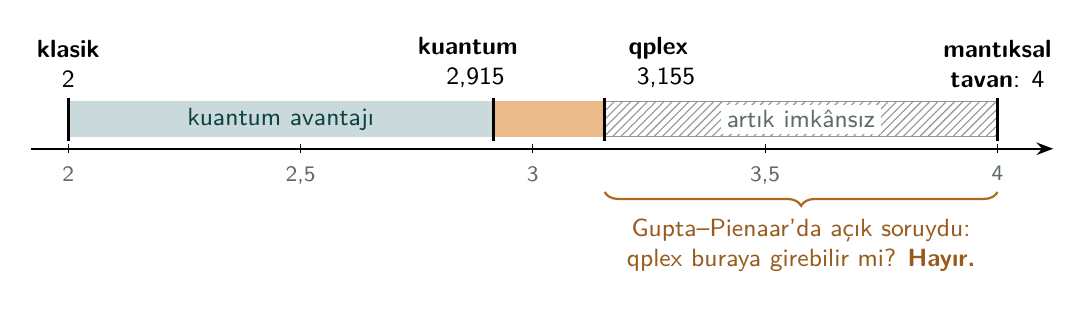
\begin{tikzpicture}[x=5.9cm,y=1cm,font=\sffamily\small]
  \fill[ana!22] (2,0.15) rectangle (2.9149,0.6);
  \fill[turuncu!55] (2.9149,0.15) rectangle (3.1547,0.6);
  \fill[pattern=north east lines,pattern color=gri!70] (3.1547,0.15) rectangle (4,0.6);
  \draw[gri!70] (3.1547,0.15) rectangle (4,0.6);
  \node[ana!80!black] at (2.457,0.375) {kuantum avantajı};
  \node[fill=white,inner sep=2pt,text=gri] at (3.577,0.375) {artık imkânsız};
  \draw[-{Stealth[length=6pt]},thick] (1.92,0)--(4.12,0);
  \foreach \v/\t in {2/2,2.5/{2,5},3/3,3.5/{3,5},4/4} \draw (\v,0.06)--(\v,-0.06) node[below=1pt,text=gri]{\footnotesize\t};
  \foreach \v in {2,2.9149,3.1547,4} \draw[very thick] (\v,0.1)--(\v,0.65);
  \node[above,align=center] at (2,0.65) {\textbf{klasik}\\2};
  \node[above,align=center] at (2.86,0.65) {\textbf{kuantum}\\≈ 2,915};
  \node[above,align=center] at (3.27,0.65) {\textbf{qplex}\\≈ 3,155};
  \node[above,align=center] at (4,0.65) {\textbf{mantıksal}\\\textbf{tavan}: 4};
  \draw[decorate,decoration={brace,amplitude=5pt,mirror},thick,turuncu!80!black] (3.1547,-0.55)--(4,-0.55)
     node[midway,below=6pt,align=center,text=turuncu!70!black]{Gupta–Pienaar'da açık soruydu:\\qplex buraya girebilir mi? \textbf{Hayır.}};
\end{tikzpicture}
\caption{CGLMP oyununda farklı teorilerin ulaşabildiği en yüksek puanlar.}
\end{figure}

%==========================================================
\section{QBism ve qplex: Kuantumu olasılıklardan yeniden kurmak}

\textbf{QBism}, kuantum mekaniğini yorumlamanın bir yolu. Bu görüşe göre bir kuantum durumu, ölçüm yapacak
kişinin gelecekteki sonuçlar hakkındaki \emph{kişisel olasılık beklentileridir}. Kuantum mekaniğinin
temel olasılık kuralı (Born kuralı) ise bu beklentilerin birbiriyle tutarlı olması için bir kuraldır. Bu
bakış açısından doğan iddialı bir soru var: Olasılık listelerine birkaç basit geometrik kural koyarsak,
kuantum teorisinin tamamı kendiliğinden ortaya çıkar mı?

Bu kurallara uyan olasılık kümelerine \textbf{qplex} deniyor. Üç seviyeli bir sistem için her durum 9
sayılık bir olasılık listesi. Kural şaşırtıcı derecede sade: Herhangi iki liste ne çok benzer ne de çok
farklı olabilir. Sayısal olarak, iki listenin iç çarpımı $1/12$ ile $1/6$ arasında kalmalı.

\begin{sezgi}[Gupta ve Pienaar ne buldu?]
İki kişilik korelasyonları qplex diliyle yazdılar. İki cevaplı CHSH testinde qplex kuralları tam
olarak kuantum sınırını (Tsirelson sınırı, $2\sqrt2$) veriyor. Bu, programın bir başarısı. Ama üç
cevaplı CGLMP testinde qplex'ler 3,1547'ye ulaşabiliyor, yani kuantumdan fazlasına. Demek ki qplex
kuralları tek başına yetmiyor, ek fiziksel ilkeler gerekiyor. Peki qplex'ler en fazla ne kadar ileri
gidebilir? Makalelerinin ilk sürümünde mantıksal tavan 4'e kadar çıkabildiklerini yazmışlar, sonra bunun
hatalı olduğunu belirtip düzeltmişler. İkinci sürümde soru açık kaldı.
\end{sezgi}

%==========================================================
\section{Ne kanıtladık?}

\begin{sonuc}
{\sffamily\bfseries\color{ana} Ana sonuç.} Hangi ağırlıklar, hangi başlangıç durumu ve hangi qplex seçilirse
seçilsin, Gupta–Pienaar modelindeki CGLMP puanı
\[
  T_\star \;=\; 2+\frac{2}{\sqrt3}\;\approx\;3{,}1547
\]
değerini geçemez. Bu değere ancak Alice'in sonuçları eşit olasılıklıyken ulaşılabilir.
\end{sonuc}

Buradaki \textbf{ağırlıklar}, modelin serbest ayarları: Alice'in her sonucu ne sıklıkla aldığı ve Bob'un
ölçümünün yapısı. Gupta ve Pienaar'ın örneğinde her şey eşit (“yansız”). Asıl zorluk ağırlıklar eşit
olmadığında başlıyor. Simetri bozulunca zarif matematiksel kısayollar çalışmaz hâle geliyor. Yol boyunca
şu sonuçlar çıktı:

\begin{enumerate}[leftmargin=*]
  \item \textbf{Eşit ağırlıklar için kısa, zarif bir kanıt.} Bir Fourier dönüşümü problemi 4×4'lük bir
        matrise indiriyor. Ortaya çıkan “sertifika” bir izdüşüm matrisi ve kâğıt kalemle kontrol edilebiliyor.
  \item \textbf{Fizikteki bir ilkeyle şaşırtıcı bir çakışma.} \emph{Makroskopik yerellik} adlı bir ilke var:
        Çok sayıda parçacığın ortalama davranışı klasik görünmeli. Bu ilkenin CGLMP için izin verdiği tavan da
        tam olarak 3,1547. Eşit ağırlıklı bütün qplex korelasyonlarının bu ilkeye uyduğunu gösterdik. Yani bu
        sayı bir tesadüf değil.
  \item \textbf{Bir sürpriz.} Ağırlıklar eşit olmadığında, makroskopik yerelliği \emph{ihlal eden} bir qplex
        korelasyonu bulduk. Tam kesirlerle yazılmış 12 olasılık listesi ve bunu kanıtlayan 9×9'luk bir tamsayı
        matrisi var. Demek ki qplex dünyası bu ilkenin içine sığmıyor, ama yine de aynı tavanı aşamıyor. Bu
        yüzden genel kanıt için başka bir yol gerekti.
  \item \textbf{“Neredeyse kuantum” ile karşılaştırma.} Gupta–Pienaar'ın örneği, fizikçilerin “neredeyse
        kuantum” dediği daha dar kümenin dışında kalıyor, çünkü o kümenin tavanı 2,915.
  \item \textbf{Genel durum: bilgisayar destekli kanıt.} Bir sonraki bölümün konusu.
\end{enumerate}

%==========================================================
\section{Bilgisayar destekli kanıt nasıl çalışıyor?}

Ağırlıkların alabileceği bütün değerler dört boyutlu bir bölge oluşturuyor. Bu bölgeyi \textbf{874
kutuya} böldük. Bilgisayar her kutu için bir \textbf{sertifika} üretti: O kutudaki hiçbir modelin
$3{,}1547$'yi geçemeyeceğini gösteren bir sayı listesi. Sertifikayı \emph{bulmak} zor, ama \emph{kontrol
etmek} kolay. Bir sudoku çözümünü bulmak zordur ama doğru olduğunu kontrol etmek dakikalar alır. Burada da
kontrol için birkaç matrisin “pozitif” olduğunu ve birkaç sayının $T_\star$'dan küçük olduğunu doğrulamak
yetiyor.

En zor yer optimum noktanın çevresi. Orada puan $T_\star$'a çok yaklaştığı için sabit bir sertifika işe
yaramıyor. Bu yüzden optimumun etrafındaki küçük bir topta (yarıçapı $1/125$), ağırlıklar değiştikçe
kendisi de değişen “hareketli” bir sertifika kullandık.

\begin{figure}[h]
\centering
\begin{minipage}[c]{0.5\textwidth}\centering
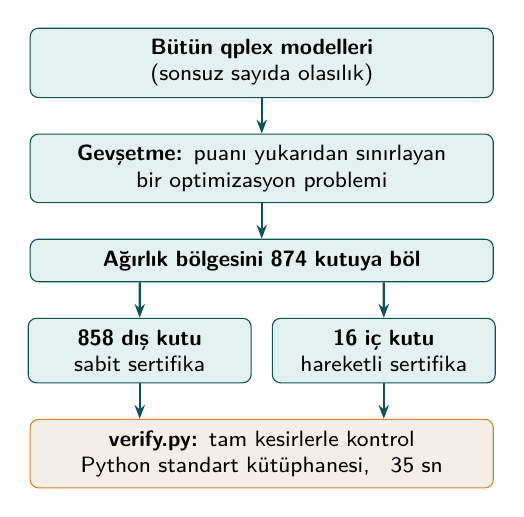
\begin{tikzpicture}[font=\sffamily\footnotesize,node distance=4.5mm,
  kutu/.style={draw=ana,fill=tur,rounded corners=3pt,align=center,text width=5.6cm,inner sep=4pt},
  ok/.style={-{Stealth[length=5pt]},thick,ana}]
  \node[kutu] (a) {\textbf{Bütün qplex modelleri}\\(sonsuz sayıda olasılık)};
  \node[kutu,below=of a] (b) {\textbf{Gevşetme:} puanı yukarıdan sınırlayan\\bir optimizasyon problemi};
  \node[kutu,below=of b] (c) {\textbf{Ağırlık bölgesini 874 kutuya böl}};
  \node[kutu,below=of c,text width=2.55cm,xshift=-1.55cm] (d1) {\textbf{858 dış kutu}\\sabit sertifika};
  \node[kutu,below=of c,text width=2.55cm,xshift=1.55cm] (d2) {\textbf{16 iç kutu}\\hareketli sertifika};
  \coordinate (m) at ($(d1.south)!0.5!(d2.south)$);
  \node[kutu,below=4.5mm of m,fill=kum,draw=turuncu] (e) {\textbf{verify.py:} tam kesirlerle kontrol\\Python standart kütüphanesi, ≈ 35 sn};
  \draw[ok] (a)--(b); \draw[ok] (b)--(c);
  \draw[ok] (c.south)++(-1.55,0)--(d1); \draw[ok] (c.south)++(1.55,0)--(d2);
  \draw[ok] (d1)--(d1|-e.north); \draw[ok] (d2)--(d2|-e.north);
\end{tikzpicture}
\end{minipage}%
\begin{minipage}[c]{0.46\textwidth}\centering
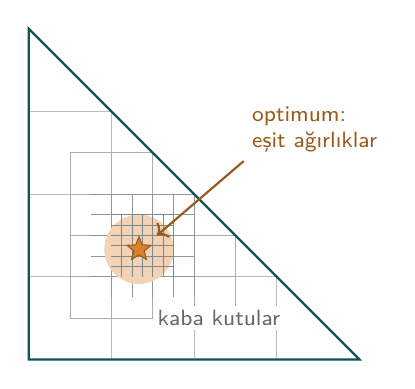
\begin{tikzpicture}[scale=1.05,font=\sffamily\footnotesize]
  \begin{scope}
    \clip (0,0)--(4,0)--(0,4)--cycle;
    \draw[gri!45] (0,0) grid (4,4);
    \draw[gri!55,step=0.5] (0.5,0.5) grid (2.5,2.5);
    \draw[gri!70,step=0.25] (0.75,0.75) grid (2,2);
    \fill[turuncu!35] (4/3,4/3) circle (0.42);
    \draw[gri!80,step=0.125] (1,1) grid (1.75,1.75);
  \end{scope}
  \draw[thick,ana] (0,0)--(4,0)--(0,4)--cycle;
  \node[star,star points=5,star point ratio=2.3,fill=turuncu,draw=turuncu!70!black,inner sep=1.4pt] at (4/3,4/3) {};
  \draw[<-,thick,turuncu!70!black] (1.55,1.5)--(2.6,2.4) node[above right=-1pt,align=left,text=turuncu!70!black]{optimum:\\eşit ağırlıklar};
  \node[gri,fill=white,inner sep=1.5pt] at (2.3,0.5) {kaba kutular};
\end{tikzpicture}\\[2pt]
{\footnotesize\color{gri} Temsilî iki boyutlu kesit. Gerçek bölge dört\\boyutlu. Optimuma yaklaştıkça kutular küçülüyor.}
\end{minipage}
\caption{Bilgisayar destekli kanıtın akışı (solda) ve kutulara bölmenin sezgisi (sağda).}
\end{figure}

\begin{sezgi}[Neden güvenilir?]
Kontrollerin hiçbiri ondalıklı sayılarla yapılmıyor. Her şey tam kesirlerle ve $a+b\sqrt3$ biçimindeki
sayılarla hesaplanıyor, yani yuvarlama hatasına yer yok. Kontrol programı sadece Python'un standart
kütüphanesini kullanıyor ve hiçbir optimizasyon yazılımına güvenmiyor. Kutuların bütün bölgeyi
kenarları dahil eksiksiz kapladığı da tam aritmetikle doğrulanıyor.
\end{sezgi}

\begin{center}
\begin{tabular}{@{}r@{\hspace{10pt}}l@{}}
\toprule
\textbf{874} & kutu (858 dış + 16 iç) \\
\textbf{118} & sayı: her kutunun sertifikası \\
\textbf{≈ 2 milyonda 1} & dış kutulardaki en yüksek puanın $T_\star$'a kalan mesafesi (oransal olarak) \\
\textbf{1/125} & optimum etrafındaki hareketli sertifikanın yarıçapı \\
\textbf{≈ 35 saniye} & bütün kontrollerin sıradan bir dizüstü bilgisayarda sürdüğü zaman \\
\bottomrule
\end{tabular}
\end{center}

%==========================================================
\section{Ne kadar güvenebiliriz?}

Sonuç birbirinden ayrı yollarla denetlendi. OpenAI Codex kanıtları gözden geçirip ayrı bir doğrulayıcı
yazdı ve makaleyi revize etti. Gemini makaleyi değerlendirip iyileştirme önerileri verdi. Claude da son
sürümü bir hakem gibi denetledi: Her adımı, kendi sıfırdan yazdığı ayrı kodla ve kutuların bölgeyi
kapladığını farklı bir yöntemle kontrol ederek yeniden hesapladı. Bütün kontroller aynı sonucu verdi.

\begin{dikkat}[Dürüst olmak gerekirse]
\begin{itemize}[leftmargin=*]
  \item Sonucu henüz hiçbir insan uzman incelemedi ve hakemli bir dergide yayımlanmadı.
  \item Kanıtın ilk adımı, Gupta–Pienaar modelini doğru okuduğumuz varsayımına dayanıyor. Bu adım en çok
        şüpheyle bakılmayı hak eden yer.
  \item Yöntemi ve ilk kodu Claude ürettiği için Claude'un yaptığı denetim tam anlamıyla bağımsız sayılmaz.
\end{itemize}
Bu nedenle makale, modelin yazarlarından Jacques Pienaar'a iletildi.
\end{dikkat}

%==========================================================
\section{Bu neden önemli?}

\begin{itemize}[leftmargin=*]
  \item \textbf{QBism programı için net bir sayı.} Qplex kurallarının CGLMP testinde kuantumdan ne kadar
        fazlasına izin verdiği artık tam olarak biliniyor: 3,1547'ye kadar, ne eksik ne fazla. Kuantum
        teorisine ulaşmak için eklenecek ilke, 3,1547 ile 2,915 arasındaki farkı kapatmalı.
  \item \textbf{Fizikteki ilkelerle beklenmedik bir bağlantı.} Tavanın makroskopik yerellikle aynı çıkması,
        qplex geometrisi ile bu ilke arasında derin bir ilişki olabileceğini düşündürüyor. Eşit olmayan
        ağırlıklı örnek ise bu ilişkinin basit bir “biri ötekinin içinde” ilişkisi olmadığını gösteriyor.
  \item \textbf{Yeni sorular.} Dört cevaplı oyunda ne olur? Orada makroskopik yerelliğin tavanı yaklaşık
        3,2126. Ayrıca iki ayrı sistemden kurulmuş gerçek bir qplex modeli bu korelasyonları üretebilir mi?
\end{itemize}

%==========================================================
\section{Kim ne yaptı?}

\renewcommand{\arraystretch}{1.25}
\begin{tabularx}{\textwidth}{@{}>{\raggedright\bfseries}p{5.4cm}>{\raggedright\arraybackslash}X@{}}
\toprule
Yusuf Kaan Öğüt & Soruyu seçti, problemi eşit olmayan ağırlıklara genişletmeyi önerdi, süreci yönetti ve
                  makalenin sorumluluğunu taşıyor. \\
Claude Opus 5.5 (Anthropic) & İlk kanıtları, bilgisayar aramasını, sertifikaları ve ilk taslağı üretti.
                  Son sürümü hakem gibi denetledi. \\
OpenAI Codex (GPT-6.2 Astra) & Kanıtları gözden geçirdi, ayrı bir doğrulayıcı yazdı, zarif izdüşüm
                  biçimini ve kesirli örneği buldu, makaleyi revize etti. \\
Gemini 4 Neon & Makaleyi bağımsız olarak değerlendirdi ve öneriler verdi. \\
\bottomrule
\end{tabularx}

\begin{sezgi}[Kendin dene]
Teknik makale, bütün sertifikalar ve kodlar GitHub'da herkese açık:\par
\href{https://github.com/basketktri-ux/qplex-cglmp-optimal-bound}{\color{ana}\texttt{github.com/basketktri-ux/qplex-cglmp-optimal-bound}}\par
Kontrol etmek için depoyu indirip ana klasörde şu komutu çalıştırman yeterli, ek kurulum gerekmiyor:\par
\texttt{python3 certificate/verify.py}
\end{sezgi}

\subsection*{Kaynaklar}
{\small
\begin{itemize}[leftmargin=*,itemsep=1pt]
  \item S. Gupta ve J. Pienaar, \emph{Quantum correlations in QBism's reconstruction program}, arXiv:2606.07485 (2026).
  \item M. Appleby, C. A. Fuchs, B. C. Stacey ve H. Zhu, \emph{Introducing the qplex}, Eur. Phys. J. D 71, 197 (2017).
  \item D. Collins, N. Gisin, N. Linden, S. Massar ve S. Popescu, \emph{Bell inequalities for arbitrarily high-dimensional systems}, Phys. Rev. Lett. 88, 040404 (2002).
  \item M. Navascués ve H. Wunderlich, \emph{A glance beyond the quantum model}, Proc. R. Soc. A 466, 881 (2010).
  \item Y. K. Öğüt, \emph{The optimal three-outcome CGLMP value in the Gupta–Pienaar qplex model}, teknik makale (2026).
\end{itemize}}

\end{document}
